\chapter{Theoretische Grundlagen}

\section{Begriffsdefinitionen}
In den folgenden Kapiteln werden die Begriffe „Social Network Analysis“, „Graph“ und „Link-Prediction“ einzeln
erläutert. Es handelt sich in Bezug auf die Arbeit um grundlegende Begriffe. Weitere Fachbegriffe, die
in der Arbeit verwendet werden, sind im Glossar beschrieben.
% TODO Make glossary

\subsection{Social Network Analysis}
Soziale Netzwerke bestehen aus Akteuren, wie beispielsweise Individuen, Organisationen oder ganze Nationen und deren Beziehungen.\cite{noauthor_soziale_nodate}.
Unter \acl{sna} (SNA, dt. Soziale Netzwerkanalyse) wird die Methode zur Erfassung und Analyse von dieser Netzwerke und der Beziehungen darin verstanden \cite{noauthor_soziale_2019}.
Die soziale Netzwerkanalyse ist ein interdisziplinäres Forschungsfeld und wird in den Sozial- und Verhaltenswissenschaften aber auch in der Betriebswirtschaftslehre oder den Politikwissenschafften angewandt \cite{noauthor_soziale_nodate}.
Gegenwärtig sind sogenannte "soziale Netzwerke" allgegenwärtig und werden insbesondere im Kontext von Internet-Plattformen wie \textit{Facebook} oder \textit{Twitter} häufig betrachtet.

\subsection{Graph}
Soziale Netzwerke können einfach als Graph modelliert werden.
Ein Graph $G = (V, E)$ besteht aus einer Menge $V = \{1,2,...,|V|\}$ von Knoten und Kanten $E \subseteq V\times V $(vgl. \cite{ottmann_algorithmen_2017}).
Die Knoten repräsentieren dabei Akteure, während die Kanten die Beziehungen zwischen den Akteuren repräsentieren.
Abbildung \ref{fig:graph_ungerichtet} zeigt einen ungerichteten Graphen. Die Kanten enthalten dabei keine Pfeile, was verdeutlicht, dass die Interaktion in beide Richtungen erfolgen kann.
Ein Beispiel für einen ungerichteten Graphen ist das Freundes-Netzwerk von \textit{Facebook}.

\begin{figure}[h]
    \centering
    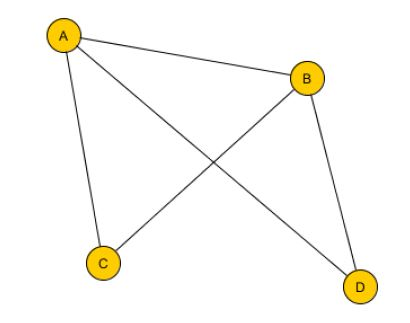
\includegraphics{resources/img_graph_undirected.JPG}
    \caption{Ungerichteter Graph}
    % TODO Add cite to SNA Script
    \label{fig:graph_undirected}
\end{figure}

Im Gegensatz dazu gibt es bei einem gerichteten Graphen eine Quelle und ein Ziel. Die Richtung der Interaktion wird durch einen Pfeil visualisiert.
Abbildung \ref{fig:graph_directed} zeigt einen solchen Graphen.
Als Beispiel für einen gerichteten Graphen dient ein E-Mail Netzwerk. Jede Nachricht wird dabei von einem Sender an einen Empfänger versendet.

\begin{figure}[h]
    \centering
    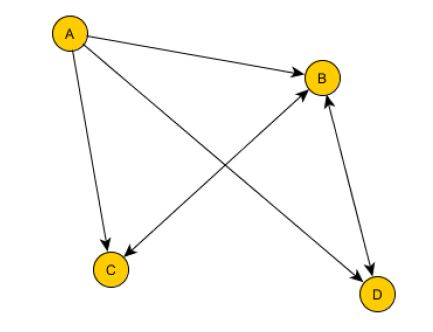
\includegraphics{resources/img_graph_directed.JPG}
    \caption{Gerichteter Graph}
    % TODO Add cite to SNA Script
    \label{fig:graph_directed}
\end{figure}

\subsection{Link-Prediction}
\cite{gao_link_2015}

Dummy text.
